\section{Problem 1}
\label{sec:problem1}

First, define the following:
\begin{equation*}
R=\frac{r_2}{r_1},\qquad S=\frac{r_i}{r_2},\qquad v_{c1}=\sqrt{\frac{\mu}{r_1}}
\end{equation*}

\subsection*{(a) Hohmann transfer}

The equations for the Hohmann transfer are
\begin{align*}
a &= \frac{r_1+r_2}{2}\\[4pt]
\Delta v_1 &= \sqrt{\frac{2\mu}{r_1}-\frac{\mu}{a}} - \sqrt{\frac{\mu}{r_1}}
  = \sqrt{\frac{\mu}{r_1}}\left(\sqrt{\frac{2r_2}{r_1+r_2}}-1\right)\\[4pt]
\Delta v_2 &= \sqrt{\frac{\mu}{r_2}} - \sqrt{\frac{2\mu}{r_2}-\frac{\mu}{a}}
  = \sqrt{\frac{\mu}{r_2}}\left(1-\sqrt{\frac{2r_1}{r_1+r_2}}\right)
\end{align*}
Nondimensionalizing by $v_{c1}$ with $r_2 = Rr_1$, we get
\begin{equation}
\boxed{\frac{\Delta v_1}{v_{c1}} = \sqrt{\frac{2R}{1+R}} - 1, \qquad
\frac{\Delta v_2}{v_{c1}} = \sqrt{\frac{1}{R}} - \sqrt{\frac{2}{R(1+R)}}}
\label{eq:p1-hohmann}
\end{equation}

\subsection*{(b) Bi-elliptic transfer}

The equations for the bi-elliptic transfer are
\begin{align*}
a_1 &= \frac{r_1+r_i}{2}, \qquad a_2 = \frac{r_2+r_i}{2}\\[4pt]
\Delta v_1 &= \sqrt{\frac{2\mu}{r_1}-\frac{\mu}{a_1}} - \sqrt{\frac{\mu}{r_1}}
  = \sqrt{\frac{\mu}{r_1}}\left(\sqrt{\frac{2r_i}{r_1+r_i}}-1\right)\\[4pt]
\Delta v_2 &= \sqrt{\frac{2\mu}{r_i}-\frac{\mu}{a_2}} - \sqrt{\frac{2\mu}{r_i}-\frac{\mu}{a_1}}
  = \sqrt{\frac{\mu}{r_i}}\left(\sqrt{\frac{2r_2}{r_2+r_i}}-\sqrt{\frac{2r_1}{r_1+r_i}}\right)\\[4pt]
\Delta v_3 &= \sqrt{\frac{2\mu}{r_2}-\frac{\mu}{a_2}} - \sqrt{\frac{\mu}{r_2}}
  = \sqrt{\frac{\mu}{r_2}}\left(\sqrt{\frac{2r_i}{r_2+r_i}}-1\right)
\end{align*}
Nondimensionalizing by $v_{c1}$ with $r_2 = Rr_1$ and $r_i = RSr_1$, we get
\begin{equation}
\boxed{
\begin{gathered}
\frac{\Delta v_1}{v_{c1}} = \sqrt{\frac{2RS}{1+RS}} - 1, \qquad
\frac{\Delta v_2}{v_{c1}} = \sqrt{\frac{1}{RS}}\left(\sqrt{\frac{2}{1+S}} - \sqrt{\frac{2}{1+RS}}\right), \\[4pt]
\frac{\Delta v_3}{v_{c1}} = \sqrt{\frac{2S}{R+RS}} - \sqrt{\frac{1}{R}}
\end{gathered}}
\label{eq:p1-bielliptic}
\end{equation}

\Needspace{16\baselineskip}
\subsection*{(c) Bi-parabolic transfer}

The bi-parabolic transfer is the limit $S\to\infty$ of the nondimensional bi-elliptic impulses:
\begin{alignat*}{2}
\frac{\Delta v_1}{v_{c1}} &= \sqrt{\frac{2R}{1/S+R}} - 1
  &&\qquad\xrightarrow{S\to\infty}\quad \sqrt{2}-1\\[4pt]
\frac{\Delta v_2}{v_{c1}} &= \sqrt{\frac{1}{RS}}\left(\sqrt{\frac{2/S}{1/S+1}} - \sqrt{\frac{2/S}{1/S+R}}\right)
  &&\qquad\xrightarrow{S\to\infty}\quad 0\\[4pt]
\frac{\Delta v_3}{v_{c1}} &= \sqrt{\frac{2}{R/S+R}} - \sqrt{\frac{1}{R}}
  &&\qquad\xrightarrow{S\to\infty}\quad \left(\sqrt{2}-1\right)\sqrt{\frac{1}{R}}
\end{alignat*}
This leaves us with two impulses:
\begin{equation}
\boxed{\frac{\Delta v_1}{v_{c1}} = \sqrt{2}-1, \qquad \frac{\Delta v_2}{v_{c1}} = \left(\sqrt{2}-1\right)\sqrt{\frac{1}{R}}}
\label{eq:p1-biparabolic}
\end{equation}

\subsection*{(d) Comparison plots}

Equations~\eqref{eq:p1-hohmann}, \eqref{eq:p1-bielliptic}, and \eqref{eq:p1-biparabolic} are implemented in \texttt{transfers.py} and evaluated in \texttt{problem1.py} with $S\in\{2,5,10,11,12,15\}$. \Cref{fig:p1-full} shows $\Delta v/v_{c1}$ for $R\in[1,20]$ and \cref{fig:p1-zoom} the enlarged view for $R\in[10,16]$, $\Delta v/v_{c1}\in[0.51,0.55]$.

\begin{figure}[H]
\centering
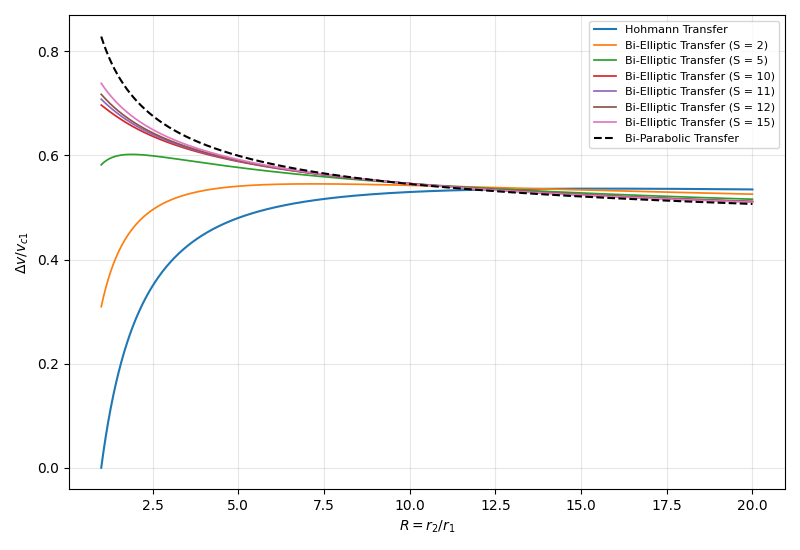
\includegraphics[width=0.85\textwidth]{problem1_full.png}
\caption{Normalized total impulse $\Delta v/v_{c1}$ vs.\ $R=r_2/r_1$ for $R\in[1,20]$.}
\label{fig:p1-full}
\end{figure}

\begin{figure}[H]
\centering
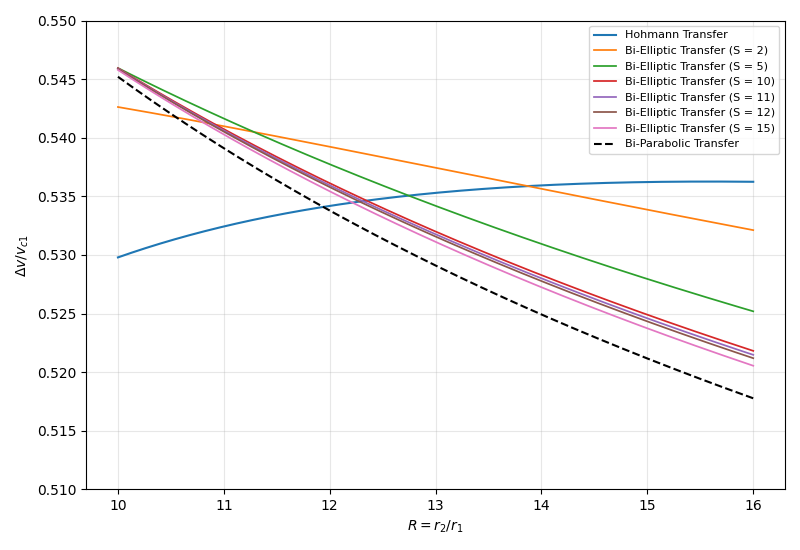
\includegraphics[width=0.85\textwidth]{problem1_zoom.png}
\caption{Enlarged view for $R\in[10,16]$, $\Delta v/v_{c1}\in[0.51,0.55]$.}
\label{fig:p1-zoom}
\end{figure}

\FloatBarrier
